\documentclass[]{article}
\usepackage{lmodern}
\usepackage{amssymb,amsmath}
\usepackage{ifxetex,ifluatex}
\usepackage{fixltx2e} % provides \textsubscript
\ifnum 0\ifxetex 1\fi\ifluatex 1\fi=0 % if pdftex
  \usepackage[T1]{fontenc}
  \usepackage[utf8]{inputenc}
\else % if luatex or xelatex
  \ifxetex
    \usepackage{mathspec}
    \usepackage{xltxtra,xunicode}
  \else
    \usepackage{fontspec}
  \fi
  \defaultfontfeatures{Mapping=tex-text,Scale=MatchLowercase}
  \newcommand{\euro}{€}
\fi
% use upquote if available, for straight quotes in verbatim environments
\IfFileExists{upquote.sty}{\usepackage{upquote}}{}
% use microtype if available
\IfFileExists{microtype.sty}{%
\usepackage{microtype}
\UseMicrotypeSet[protrusion]{basicmath} % disable protrusion for tt fonts
}{}
\usepackage[margin=1in]{geometry}
\ifxetex
  \usepackage[setpagesize=false, % page size defined by xetex
              unicode=false, % unicode breaks when used with xetex
              xetex]{hyperref}
\else
  \usepackage[unicode=true]{hyperref}
\fi
\hypersetup{breaklinks=true,
            bookmarks=true,
            pdfauthor={},
            pdftitle={The Exponential Distribution in R versus the Central Limit Theorem},
            colorlinks=true,
            citecolor=blue,
            urlcolor=blue,
            linkcolor=magenta,
            pdfborder={0 0 0}}
\urlstyle{same}  % don't use monospace font for urls
\usepackage{color}
\usepackage{fancyvrb}
\newcommand{\VerbBar}{|}
\newcommand{\VERB}{\Verb[commandchars=\\\{\}]}
\DefineVerbatimEnvironment{Highlighting}{Verbatim}{commandchars=\\\{\}}
% Add ',fontsize=\small' for more characters per line
\usepackage{framed}
\definecolor{shadecolor}{RGB}{248,248,248}
\newenvironment{Shaded}{\begin{snugshade}}{\end{snugshade}}
\newcommand{\KeywordTok}[1]{\textcolor[rgb]{0.13,0.29,0.53}{\textbf{{#1}}}}
\newcommand{\DataTypeTok}[1]{\textcolor[rgb]{0.13,0.29,0.53}{{#1}}}
\newcommand{\DecValTok}[1]{\textcolor[rgb]{0.00,0.00,0.81}{{#1}}}
\newcommand{\BaseNTok}[1]{\textcolor[rgb]{0.00,0.00,0.81}{{#1}}}
\newcommand{\FloatTok}[1]{\textcolor[rgb]{0.00,0.00,0.81}{{#1}}}
\newcommand{\ConstantTok}[1]{\textcolor[rgb]{0.00,0.00,0.00}{{#1}}}
\newcommand{\CharTok}[1]{\textcolor[rgb]{0.31,0.60,0.02}{{#1}}}
\newcommand{\SpecialCharTok}[1]{\textcolor[rgb]{0.00,0.00,0.00}{{#1}}}
\newcommand{\StringTok}[1]{\textcolor[rgb]{0.31,0.60,0.02}{{#1}}}
\newcommand{\VerbatimStringTok}[1]{\textcolor[rgb]{0.31,0.60,0.02}{{#1}}}
\newcommand{\SpecialStringTok}[1]{\textcolor[rgb]{0.31,0.60,0.02}{{#1}}}
\newcommand{\ImportTok}[1]{{#1}}
\newcommand{\CommentTok}[1]{\textcolor[rgb]{0.56,0.35,0.01}{\textit{{#1}}}}
\newcommand{\DocumentationTok}[1]{\textcolor[rgb]{0.56,0.35,0.01}{\textbf{\textit{{#1}}}}}
\newcommand{\AnnotationTok}[1]{\textcolor[rgb]{0.56,0.35,0.01}{\textbf{\textit{{#1}}}}}
\newcommand{\CommentVarTok}[1]{\textcolor[rgb]{0.56,0.35,0.01}{\textbf{\textit{{#1}}}}}
\newcommand{\OtherTok}[1]{\textcolor[rgb]{0.56,0.35,0.01}{{#1}}}
\newcommand{\FunctionTok}[1]{\textcolor[rgb]{0.00,0.00,0.00}{{#1}}}
\newcommand{\VariableTok}[1]{\textcolor[rgb]{0.00,0.00,0.00}{{#1}}}
\newcommand{\ControlFlowTok}[1]{\textcolor[rgb]{0.13,0.29,0.53}{\textbf{{#1}}}}
\newcommand{\OperatorTok}[1]{\textcolor[rgb]{0.81,0.36,0.00}{\textbf{{#1}}}}
\newcommand{\BuiltInTok}[1]{{#1}}
\newcommand{\ExtensionTok}[1]{{#1}}
\newcommand{\PreprocessorTok}[1]{\textcolor[rgb]{0.56,0.35,0.01}{\textit{{#1}}}}
\newcommand{\AttributeTok}[1]{\textcolor[rgb]{0.77,0.63,0.00}{{#1}}}
\newcommand{\RegionMarkerTok}[1]{{#1}}
\newcommand{\InformationTok}[1]{\textcolor[rgb]{0.56,0.35,0.01}{\textbf{\textit{{#1}}}}}
\newcommand{\WarningTok}[1]{\textcolor[rgb]{0.56,0.35,0.01}{\textbf{\textit{{#1}}}}}
\newcommand{\AlertTok}[1]{\textcolor[rgb]{0.94,0.16,0.16}{{#1}}}
\newcommand{\ErrorTok}[1]{\textcolor[rgb]{0.64,0.00,0.00}{\textbf{{#1}}}}
\newcommand{\NormalTok}[1]{{#1}}
\setlength{\parindent}{0pt}
\setlength{\parskip}{6pt plus 2pt minus 1pt}
\setlength{\emergencystretch}{3em}  % prevent overfull lines
\providecommand{\tightlist}{%
  \setlength{\itemsep}{0pt}\setlength{\parskip}{0pt}}
\setcounter{secnumdepth}{0}

%%% Use protect on footnotes to avoid problems with footnotes in titles
\let\rmarkdownfootnote\footnote%
\def\footnote{\protect\rmarkdownfootnote}

%%% Change title format to be more compact
\usepackage{titling}

% Create subtitle command for use in maketitle
\newcommand{\subtitle}[1]{
  \posttitle{
    \begin{center}\large#1\end{center}
    }
}

\setlength{\droptitle}{-2em}
  \title{The Exponential Distribution in R versus the Central Limit Theorem}
  \pretitle{\vspace{\droptitle}\centering\huge}
  \posttitle{\par}
  \author{}
  \preauthor{}\postauthor{}
  \date{}
  \predate{}\postdate{}

\usepackage{graphicx} \usepackage{textalpha}

% Redefines (sub)paragraphs to behave more like sections
\ifx\paragraph\undefined\else
\let\oldparagraph\paragraph
\renewcommand{\paragraph}[1]{\oldparagraph{#1}\mbox{}}
\fi
\ifx\subparagraph\undefined\else
\let\oldsubparagraph\subparagraph
\renewcommand{\subparagraph}[1]{\oldsubparagraph{#1}\mbox{}}
\fi

\begin{document}
\maketitle

\subsection{Overview}\label{overview}

The goal of this project is to investigate the exponential distribution
in R and compare it with the Central Limit Theorem. The exponential
distribution can be simulated in R with \texttt{rexp(n,\ lambda)} where
lambda is the rate parameter. The mean of exponential distribution is
1/lambda and the standard deviation is also 1/lambda. A
\texttt{lambda\ =\ 0.2} is set for all simulations in this report. This
report will investigate the distribution of averages of 40 exponentials.

This report will illustrate via simulation and associated explanatory
text, the properties of the distribution of the mean of 40 exponentials.
This report shows:

\begin{enumerate}
\def\labelenumi{\arabic{enumi}.}
\tightlist
\item
  The sample mean as compared to the theoretical mean of the
  distribution.
\item
  How variable the sample is (via variance) when compared to the
  theoretical variance of the distribution.
\item
  How the distribution is approximately normal.
\end{enumerate}

\subsection{Simulations}\label{simulations}

\subsubsection{Sample Mean versus Theoretical
Mean}\label{sample-mean-versus-theoretical-mean}

A series of 1000 simulations will be performed to create a dataset for
which to compare the Central Limit Theorem. Each simulation contains 40
observations and the exponential distribution function will be set to
\texttt{rexp(40,\ 0.2)}.

\begin{Shaded}
\begin{Highlighting}[]
\NormalTok{lambda =}\StringTok{ }\FloatTok{0.2}
\NormalTok{n =}\StringTok{ }\DecValTok{40} 
\NormalTok{nosim =}\StringTok{ }\DecValTok{1000}
\KeywordTok{set.seed}\NormalTok{(}\DecValTok{349}\NormalTok{)}
\end{Highlighting}
\end{Shaded}

The simulations are then carried out to collect the necessary data, and
the data is then plotted.

\begin{Shaded}
\begin{Highlighting}[]
\NormalTok{exp_sim <-}\StringTok{ }\NormalTok{function(n, lambda) \{}
        \KeywordTok{mean}\NormalTok{(}\KeywordTok{rexp}\NormalTok{(n,lambda))}
\NormalTok{\}}

\NormalTok{sim <-}\StringTok{ }\KeywordTok{data.frame}\NormalTok{(}\DataTypeTok{ncol=}\DecValTok{2}\NormalTok{,}\DataTypeTok{nrow=}\DecValTok{1000}\NormalTok{)}
\KeywordTok{names}\NormalTok{(sim) <-}\StringTok{ }\KeywordTok{c}\NormalTok{(}\StringTok{"Index"}\NormalTok{,}\StringTok{"Mean"}\NormalTok{)}

\NormalTok{for (i in }\DecValTok{1}\NormalTok{:nosim) \{}
        \NormalTok{sim[i,}\DecValTok{1}\NormalTok{] <-}\StringTok{ }\NormalTok{i}
        \NormalTok{sim[i,}\DecValTok{2}\NormalTok{] <-}\StringTok{ }\KeywordTok{exp_sim}\NormalTok{(n,lambda)}
\NormalTok{\}}
\end{Highlighting}
\end{Shaded}

The mean of the simulation data, n=1000

\begin{Shaded}
\begin{Highlighting}[]
\NormalTok{sample_mean <-}\StringTok{ }\KeywordTok{mean}\NormalTok{(sim$Mean)}
\NormalTok{sample_mean}
\end{Highlighting}
\end{Shaded}

\begin{verbatim}
## [1] 4.983227
\end{verbatim}

Theoretical exponential mean of the exponential distribution

\begin{Shaded}
\begin{Highlighting}[]
\NormalTok{theor_mean <-}\StringTok{ }\DecValTok{1}\NormalTok{/lambda}
\NormalTok{theor_mean}
\end{Highlighting}
\end{Shaded}

\begin{verbatim}
## [1] 5
\end{verbatim}

The simulation mean is virtually identical to the theoretical mean.

Histogram plot of the exponential distribution, n=1000

\begin{Shaded}
\begin{Highlighting}[]
\KeywordTok{hist}\NormalTok{(sim$Mean, }\DataTypeTok{breaks =} \DecValTok{100}\NormalTok{, }\DataTypeTok{prob =} \OtherTok{TRUE}\NormalTok{, }
     \DataTypeTok{main=}\StringTok{"Exponential Distribution, n=1000"}\NormalTok{, }\DataTypeTok{xlab=}\StringTok{"Spread"}\NormalTok{)}
        \KeywordTok{abline}\NormalTok{(}\DataTypeTok{v =} \NormalTok{theor_mean, }\DataTypeTok{col=} \DecValTok{3}\NormalTok{, }\DataTypeTok{lwd =} \DecValTok{2}\NormalTok{)}
        \KeywordTok{abline}\NormalTok{(}\DataTypeTok{v =} \NormalTok{sample_mean, }\DataTypeTok{col =} \DecValTok{2}\NormalTok{, }\DataTypeTok{lwd =} \DecValTok{2}\NormalTok{)}
        \KeywordTok{legend}\NormalTok{(}\StringTok{'topright'}\NormalTok{, }\KeywordTok{c}\NormalTok{(}\StringTok{"Sample Mean"}\NormalTok{, }\StringTok{"Theoretical Mean"}\NormalTok{), }\DataTypeTok{bty =} \StringTok{"n"}\NormalTok{,       }
                \DataTypeTok{lty =} \KeywordTok{c}\NormalTok{(}\DecValTok{1}\NormalTok{,}\DecValTok{1}\NormalTok{), }\DataTypeTok{col =} \KeywordTok{c}\NormalTok{(}\DataTypeTok{col =} \DecValTok{3}\NormalTok{, }\DataTypeTok{col =} \DecValTok{2}\NormalTok{))}
\end{Highlighting}
\end{Shaded}

\begin{center}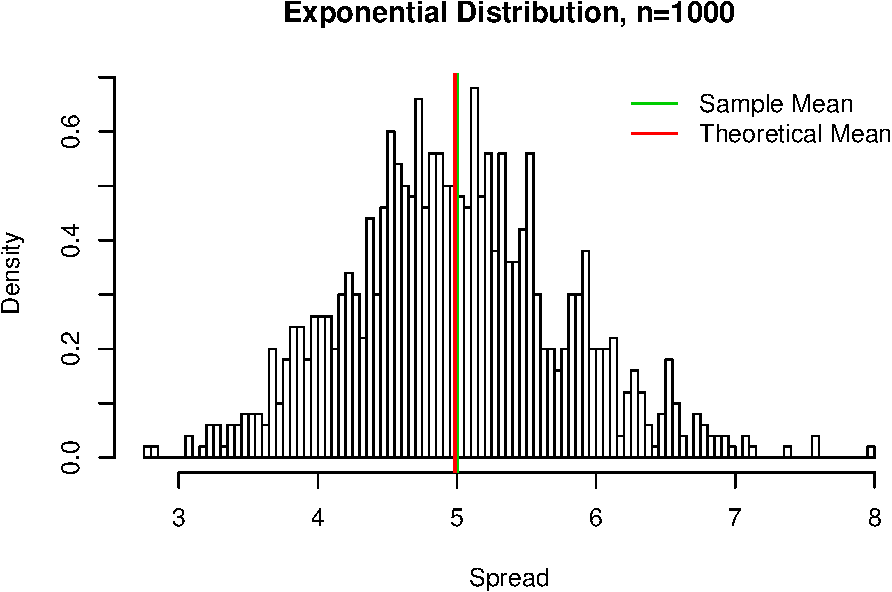
\includegraphics{part1_files/figure-latex/hist1-1} \end{center}

\subsubsection{Sample Variance versus Theoretical
Variance}\label{sample-variance-versus-theoretical-variance}

Let us now compare the variance present in the sample means of the 1000
simulations to the theoretical varience of the population.

The variance of the sample means estimates the variance of the
population by using the varience of the 1000 entries in the means vector
times the sample size, 40. In other words,
\texttt{σ2=Var(samplemeans)×N}.

\begin{Shaded}
\begin{Highlighting}[]
\NormalTok{sample_var <-}\StringTok{ }\KeywordTok{var}\NormalTok{(sim$Mean)}
\NormalTok{theor_var <-}\StringTok{ }\NormalTok{((}\DecValTok{1}\NormalTok{/lambda)^}\DecValTok{2}\NormalTok{)/}\DecValTok{40}
\end{Highlighting}
\end{Shaded}

The theoretical variance of the population is given as
\texttt{σ2=(1/lambda)2}

\begin{Shaded}
\begin{Highlighting}[]
\NormalTok{sample_var}
\end{Highlighting}
\end{Shaded}

\begin{verbatim}
## [1] 0.6010593
\end{verbatim}

\begin{Shaded}
\begin{Highlighting}[]
\NormalTok{theor_var}
\end{Highlighting}
\end{Shaded}

\begin{verbatim}
## [1] 0.625
\end{verbatim}

\begin{Shaded}
\begin{Highlighting}[]
\KeywordTok{hist}\NormalTok{(sim$Mean, }\DataTypeTok{breaks =} \DecValTok{100}\NormalTok{, }\DataTypeTok{prob =} \OtherTok{TRUE}\NormalTok{, }
     \DataTypeTok{main =} \StringTok{"Exponential Distribution, n=1000"}\NormalTok{, }\DataTypeTok{xlab =} \StringTok{"Spread"}\NormalTok{)}
        
\NormalTok{xfit <-}\StringTok{ }\KeywordTok{seq}\NormalTok{(}\KeywordTok{min}\NormalTok{(sim$Mean), }\KeywordTok{max}\NormalTok{(sim$Mean), }\DataTypeTok{length =} \DecValTok{100}\NormalTok{)}
\NormalTok{yfit <-}\StringTok{ }\KeywordTok{dnorm}\NormalTok{(xfit, }\DataTypeTok{mean =} \DecValTok{1}\NormalTok{/lambda, }\DataTypeTok{sd =} \NormalTok{(}\DecValTok{1}\NormalTok{/lambda/}\KeywordTok{sqrt}\NormalTok{(}\DecValTok{40}\NormalTok{)))}
        \KeywordTok{lines}\NormalTok{(xfit, yfit, }\DataTypeTok{pch =} \DecValTok{22}\NormalTok{, }\DataTypeTok{col =} \DecValTok{3}\NormalTok{, }\DataTypeTok{lwd =} \DecValTok{2}\NormalTok{)}
        \KeywordTok{legend}\NormalTok{(}\StringTok{'topright'}\NormalTok{, }\KeywordTok{c}\NormalTok{(}\StringTok{"Theoretical Curve"}\NormalTok{), }\DataTypeTok{lty =} \DecValTok{1}\NormalTok{,}\DataTypeTok{lwd =} \DecValTok{2}\NormalTok{, }
                \DataTypeTok{bty =} \StringTok{"n"}\NormalTok{, }\DataTypeTok{col =} \DecValTok{3}\NormalTok{)}
\end{Highlighting}
\end{Shaded}

\begin{center}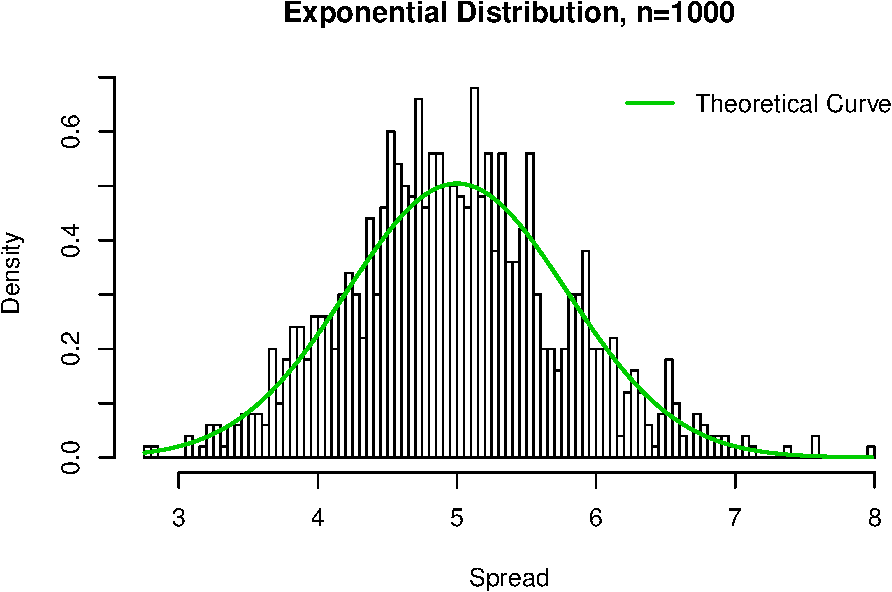
\includegraphics{part1_files/figure-latex/hist2-1} \end{center}

\begin{Shaded}
\begin{Highlighting}[]
\KeywordTok{hist}\NormalTok{(sim$Mean, }\DataTypeTok{breaks =} \DecValTok{100}\NormalTok{, }\DataTypeTok{prob =} \OtherTok{TRUE}\NormalTok{, }
     \DataTypeTok{main =} \StringTok{"Exponential Distribution, n=1000"}\NormalTok{, }\DataTypeTok{xlab =} \StringTok{"Spread"}\NormalTok{)}
        \KeywordTok{lines}\NormalTok{(}\KeywordTok{density}\NormalTok{(sim$Mean))}
        \KeywordTok{abline}\NormalTok{(}\DataTypeTok{v =} \DecValTok{1}\NormalTok{/lambda, }\DataTypeTok{col =} \DecValTok{3}\NormalTok{)}
        
\NormalTok{xfit <-}\StringTok{ }\KeywordTok{seq}\NormalTok{(}\KeywordTok{min}\NormalTok{(sim$Mean), }\KeywordTok{max}\NormalTok{(sim$Mean), }\DataTypeTok{length =} \DecValTok{100}\NormalTok{)}
\NormalTok{yfit <-}\StringTok{ }\KeywordTok{dnorm}\NormalTok{(xfit, }\DataTypeTok{mean =} \DecValTok{1}\NormalTok{/lambda, }\DataTypeTok{sd =} \NormalTok{(}\DecValTok{1}\NormalTok{/lambda/}\KeywordTok{sqrt}\NormalTok{(}\DecValTok{40}\NormalTok{))) }
        \KeywordTok{lines}\NormalTok{(xfit, yfit, }\DataTypeTok{pch =} \DecValTok{22}\NormalTok{, }\DataTypeTok{col =} \DecValTok{4}\NormalTok{, }\DataTypeTok{lty =} \DecValTok{2}\NormalTok{)}
        \KeywordTok{legend}\NormalTok{(}\StringTok{'topright'}\NormalTok{, }\KeywordTok{c}\NormalTok{(}\StringTok{"Simulated Values"}\NormalTok{, }\StringTok{"Theoretical Values"}\NormalTok{), }
                \DataTypeTok{bty =} \StringTok{"n"}\NormalTok{, }\DataTypeTok{lty =} \KeywordTok{c}\NormalTok{(}\DecValTok{1}\NormalTok{,}\DecValTok{2}\NormalTok{), }\DataTypeTok{col =} \KeywordTok{c}\NormalTok{(}\DecValTok{4}\NormalTok{, }\DecValTok{3}\NormalTok{))}
\end{Highlighting}
\end{Shaded}

\begin{center}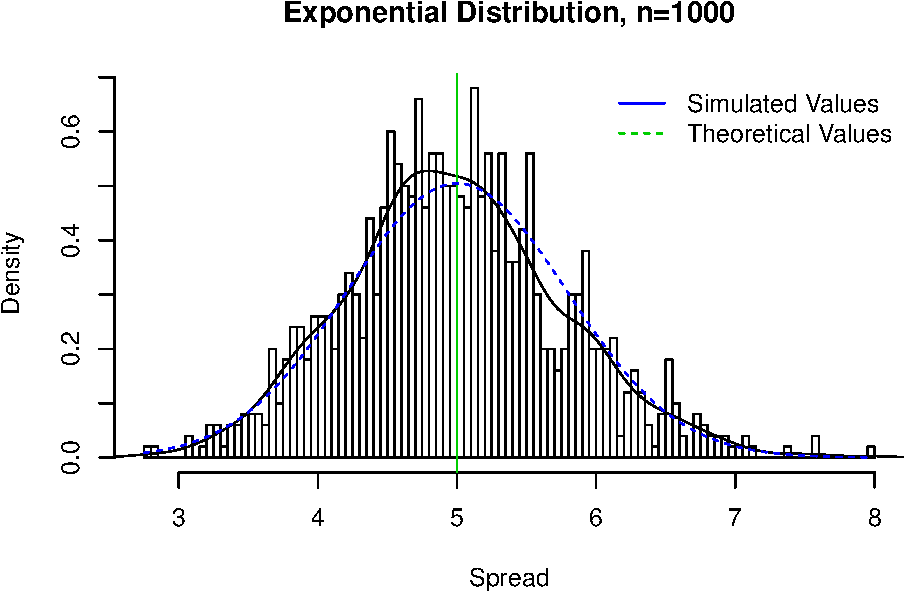
\includegraphics{part1_files/figure-latex/hist3-1} \end{center}

\subsubsection{Distribution}\label{distribution}

Due to the Central Limit Theorem, the averages of samples follow normal
distribution. The figure above also shows the density computed using the
histogram and the normal density plotted with theoretical mean and
variance values. Also, the q-q plot below suggests the normality. The
theoretical quantiles again match closely with the actual quantiles.
These four methods of comparison prove that the distribution is
approximately normal.

\begin{Shaded}
\begin{Highlighting}[]
\KeywordTok{qqnorm}\NormalTok{(sim$Mean, }\DataTypeTok{main =}\StringTok{"Normal Q-Q Plot"}\NormalTok{)}
\KeywordTok{qqline}\NormalTok{(sim$Mean, }\DataTypeTok{col =} \StringTok{"3"}\NormalTok{)}
\end{Highlighting}
\end{Shaded}

\begin{center}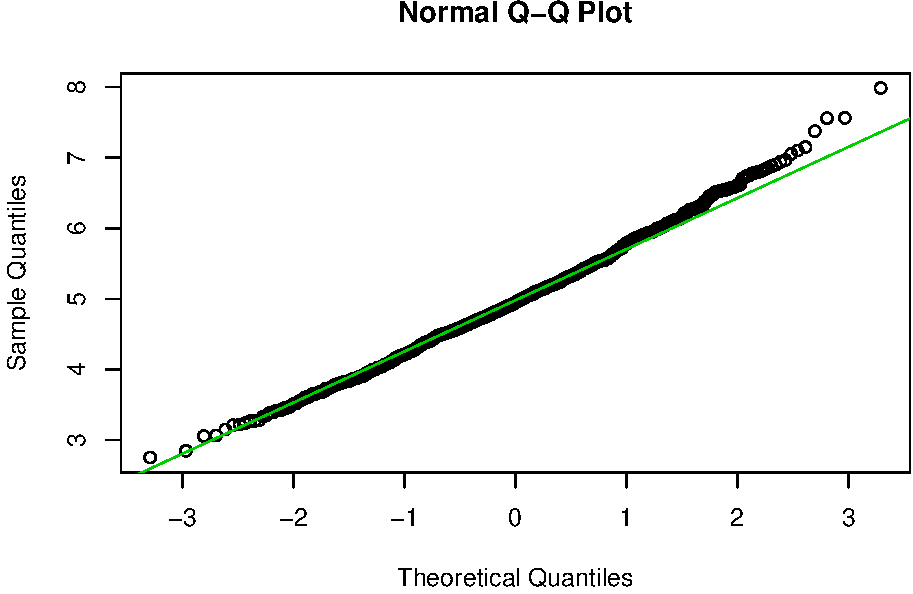
\includegraphics{part1_files/figure-latex/plot1-1} \end{center}

\end{document}
